\section{Antenna}\label{sec:antenna}
\hl{This section is not done...} So what is an antenna and why are we using it?

\subsection{Radiation patterns}
The radiation patterns is a graphical way of representing the radiation properties of the antenna as a function of space. These patterns are very useful when it comes to how an antenna perform. The antenna's pattern describes how the antenna radiates energy or how it receives energy as a function of space.

On figure \ref{fig:subfigure_RP_Dipole_Antenna}(a) is seen a simple dipole pattern which is a signal strength graph. And the pattern inside is called the azimuth pattern. In the diagram it should be seen as looking from the sky and looking down at the antenna. The numbers outside the circle represents degrees with north at the top and can be seen as a compass where north is 0$^{\circ}$, east is 90$^{\circ}$, south is 180$^{\circ}$ and west is 270$^{\circ}$. 

In this diagram the antenna is stretch from west to east which is the direction of the dipole element.  The diagram is in decibels where 0dB is at north and is the reference point. The closer we go to the center of the diagram the signal is progressively getting weaker. 0 dB is at the outer ring and is taking as the reference point. And as is moved to the center of the graph the signal is progressively getting weaker. Note that between each circle the number of the signal gets progressively smaller.

%This graph is logarithmic and non-linear (because of the increase in the signal dB).
\begin{figure}[H]
\hfill
\subfigure[Radiation pattern for a simple idealist dipole]{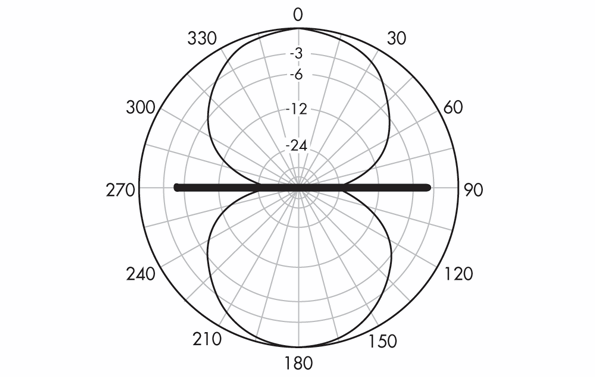
\includegraphics[width=6.5cm]{figures/radiation_pattern_dipole_antenna.png}}
\hfill
\subfigure[Dipole Antenna]{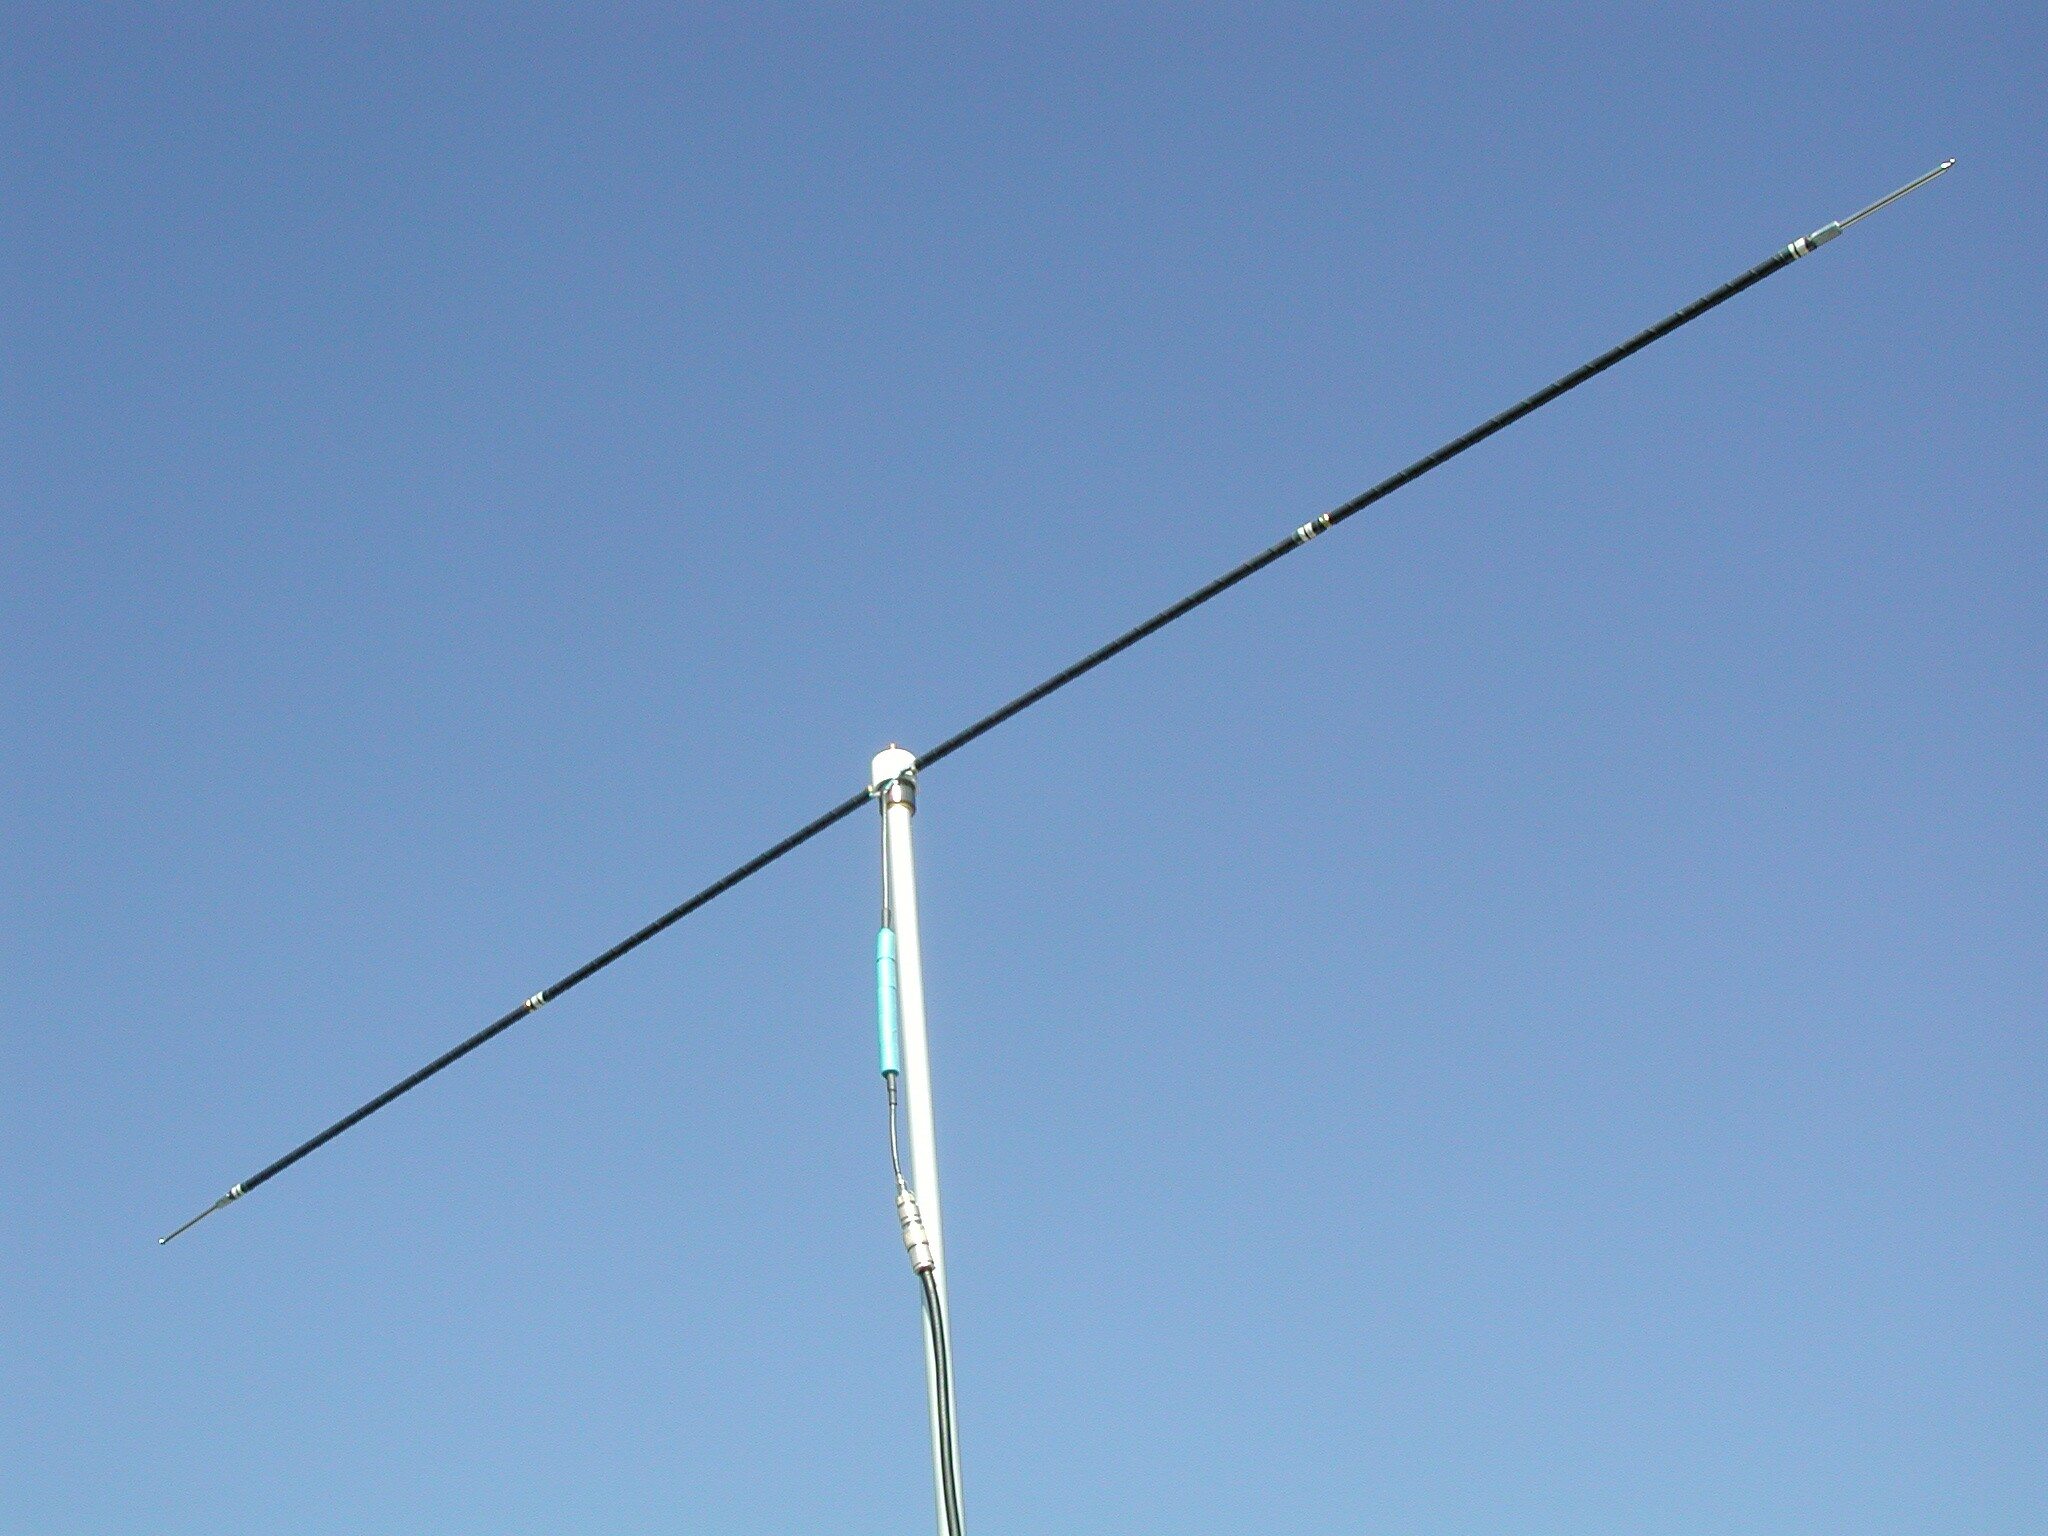
\includegraphics[width=6.5cm]{figures/dipole_antenna.jpg}}
\hfill
\caption{What are we looking at?}
\label{fig:subfigure_RP_Dipole_Antenna}
\end{figure}

\hl{Something about these figures.....}

\begin{figure}[H]
	\centering
	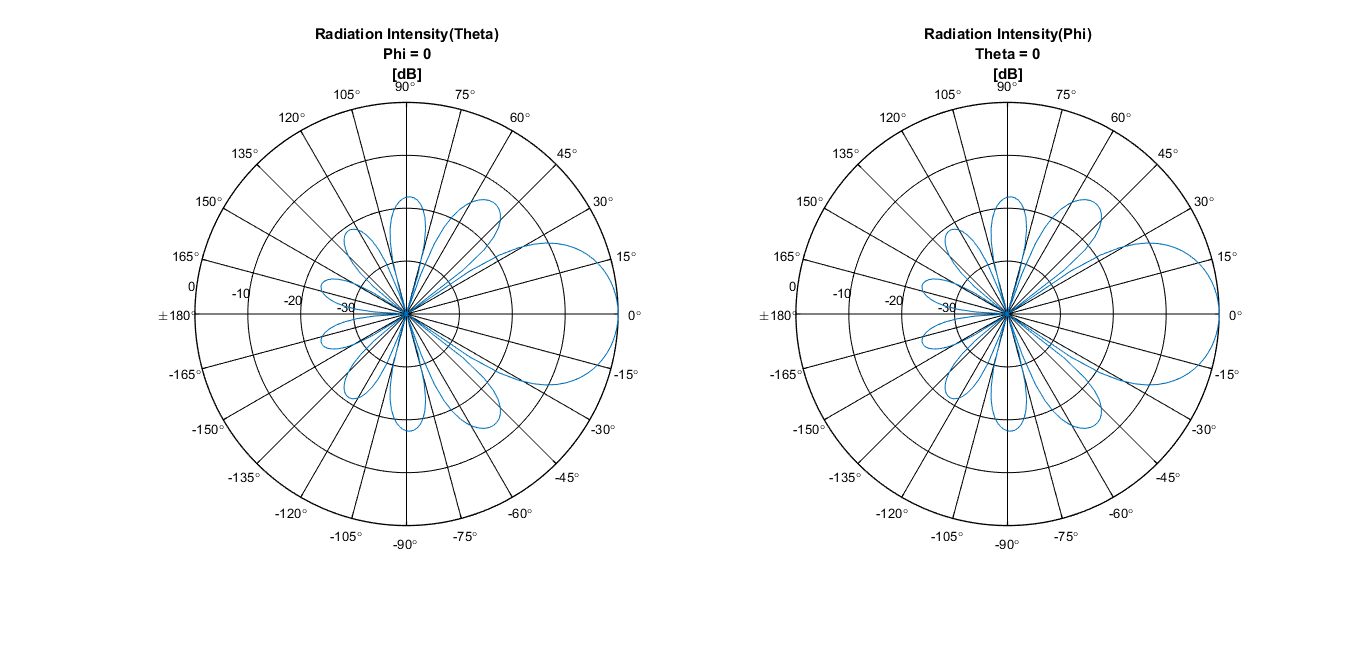
\includegraphics[scale=0.4]{figures/radiation_intensity_theta_phi.png}
	\caption{Radiation Intensity theta \& Phi}
	\label{fig:radiation_intensity_theta_phi_2}
\end{figure}

\hl{Something about these figures.....}

\begin{figure}[H]
	\centering
	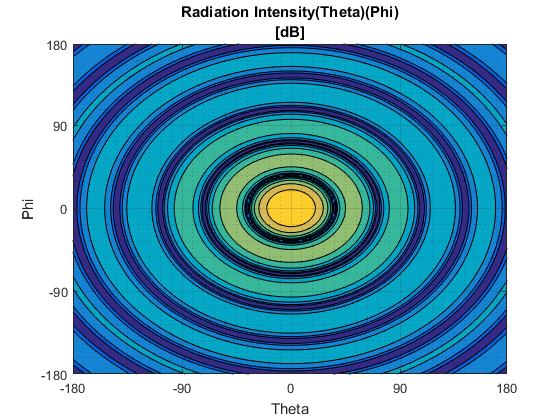
\includegraphics[scale=0.6]{figures/radiation_intensity_theta_phi_1.png}
	\caption{Radiation Intensity theta \& Phi}
	\label{fig:radiation_intensity_theta_phi_1}
\end{figure}

The radiation pattern can also be represented as a three-dimensional graph as on figure \ref{fig:radiation_pattern_3d}. 
\begin{figure}[H]
	\centering
	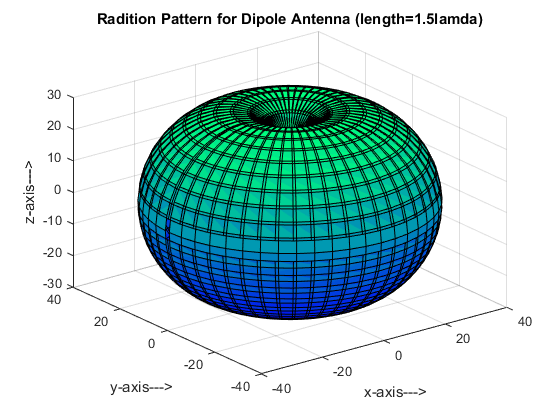
\includegraphics[scale=0.6]{figures/radiation_pattern_3d.png}
	\caption{Radiation Pattern in 3D for Dipole Antenna}
	\label{fig:radiation_pattern_3d}
\end{figure}
